%%%%%%%%%%%%%%%%%%%%%%%%%%%%%%%%%%%%%%%%%
% Beamer Presentation
% LaTeX Template
% Version 1.0 (10/11/12)
%
% This template has been downloaded from:
% http://www.LaTeXTemplates.com
%
% License:
% CC BY-NC-SA 3.0 (http://creativecommons.org/licenses/by-nc-sa/3.0/)
%
%%%%%%%%%%%%%%%%%%%%%%%%%%%%%%%%%%%%%%%%%

%----------------------------------------------------------------------------------------
%	PACKAGES AND THEMES
%----------------------------------------------------------------------------------------

\documentclass{beamer}

\mode<presentation> {

% The Beamer class comes with a number of default slide themes
% which change the colors and layouts of slides. Below this is a list
% of all the themes, uncomment each in turn to see what they look like.

%\usetheme{default}
%\usetheme{AnnArbor}
%\usetheme{Antibes}
%\usetheme{Bergen}
%\usetheme{Berkeley}
%\usetheme{Berlin}
%\usetheme{Boadilla}
%\usetheme{CambridgeUS}
%\usetheme{Copenhagen}
%\usetheme{Darmstadt}
%\usetheme{Dresden}
%\usetheme{Frankfurt}
%\usetheme{Goettingen}
%\usetheme{Hannover}
%\usetheme{Ilmenau}
%\usetheme{JuanLesPins}
%\usetheme{Luebeck}
\usetheme{Madrid}
%\usetheme{Malmoe}
%\usetheme{Marburg}
%\usetheme{Montpellier}
%\usetheme{PaloAlto}
%\usetheme{Pittsburgh}
%\usetheme{Rochester}
%\usetheme{Singapore}
%\usetheme{Szeged}
%\usetheme{Warsaw}

% As well as themes, the Beamer class has a number of color themes
% for any slide theme. Uncomment each of these in turn to see how it
% changes the colors of your current slide theme.

%\usecolortheme{albatross}
%\usecolortheme{beaver}
%\usecolortheme{beetle}
%\usecolortheme{crane}
%\usecolortheme{dolphin}
%\usecolortheme{dove}
%\usecolortheme{fly}
%\usecolortheme{lily}
%\usecolortheme{orchid}
%\usecolortheme{rose}
%\usecolortheme{seagull}
%\usecolortheme{seahorse}
%\usecolortheme{whale}
%\usecolortheme{wolverine}

%\setbeamertemplate{footline} % To remove the footer line in all slides uncomment this line
%\setbeamertemplate{footline}[page number] % To replace the footer line in all slides with a simple slide count uncomment this line

%\setbeamertemplate{navigation symbols}{} % To remove the navigation symbols from the bottom of all slides uncomment this line
}

\usepackage{graphicx} % Allows including images
\usepackage{booktabs} % Allows the use of \toprule, \midrule and \bottomrule in tables
\usepackage[T1]{fontenc}  
\usepackage[utf8]{inputenc}  
\usepackage[portuguese]{babel}
\usepackage{graphicx}
\usepackage{subfigure}
\usepackage{enumerate}
\usepackage{ae}
\usepackage{color}
\usepackage{epstopdf}

%----------------------------------------------------------------------------------------
%	TITLE PAGE
%----------------------------------------------------------------------------------------

\title[Introdução ao Processamento de Imagens]{Face Swapping} % The short title appears at the bottom of every slide, the full title is only on the title page

\author{André Nerva \\ Victória Goularte} % Your name
\institute[UnB] % Your institution as it will appear on the bottom of every slide, may be shorthand to save space
{
Universidade de Brasília  \\ % Your institution for the title page
\medskip

}
\date{\today} % Date, can be changed to a custom date

\begin{document}

\begin{frame}
\titlepage % Print the title page as the first slide
\end{frame}


%----------------------------------------------------------------------------------------
%	PRESENTATION SLIDES
%----------------------------------------------------------------------------------------

\begin{frame}
\frametitle{Introdução}
\centering
Face Swap é uma técnica de processamento de imagens  que digitalmente envolve troca de faces de dois ou mais sujeitos retratados em uma determinada fotografia.
\end{frame}

%------------------------------------------------

\begin{frame}
\frametitle{Metodologia}
\begin{itemize}
\item Leitura e redimensionamento entre duas imagens
\item Detecção dos olhos, nariz e boca 
\item Detecção das posições locais de recursos e limites nos rostos detectados
\item A partir das características foram criados pontos de destino para o mapeamento de um rosto para o outro
\item Redimensionamento e igualdade das faces na mesma posição
\item Sobreposição de faces
\item Filtro passa-baixas
\end{itemize}
\end{frame}

%------------------------------------------------

\begin{frame}
\frametitle{Leitura e redimensionamento entre duas imagens}
\centering

\begin{figure}[h]
\centering
\subfigure[Imagem base]{
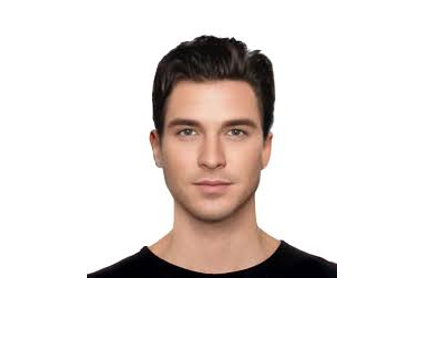
\includegraphics[scale=0.25]{imagem1.jpg}}
\subfigure[Imagem recorte]{
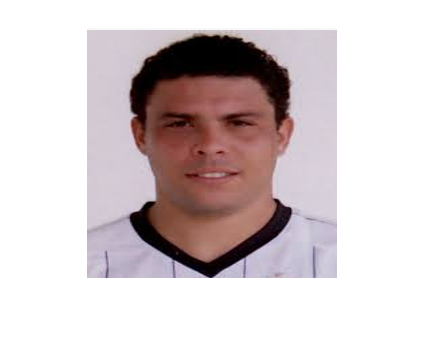
\includegraphics[scale=0.25]{imagem2.jpg}}
\end{figure}

\end{frame}

%------------------------------------------------

\begin{frame}
\frametitle{Detecção dos olhos, nariz e boca}

\begin{figure}[h]
\centering
\subfigure[Imagem detecção]{
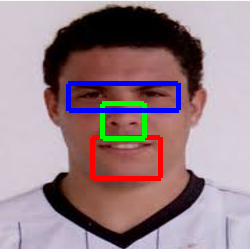
\includegraphics[scale=0.5]{deteccao.png}}
\subfigure[]{
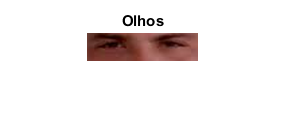
\includegraphics[scale=0.5]{olhos.png}}
\subfigure[]{
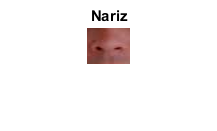
\includegraphics[scale=0.5]{nariz.png}}
\subfigure[]{
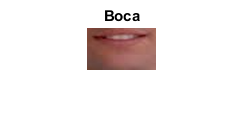
\includegraphics[scale=0.5]{boca.png}}
\end{figure}

\end{frame}

\begin{frame}
\frametitle{Detecção das posições locais de recursos e limites nos rostos detectados}

\begin{block}{Funções}
 Convex-hull\\
Detecção de Bordas\\
Preenchimento de buracos\\
\end{block}

\end{frame}


\begin{frame}
\frametitle{Detecção das posições locais de recursos e limites nos rostos detectados}
\begin{figure}[h]
\centering
\subfigure[]{
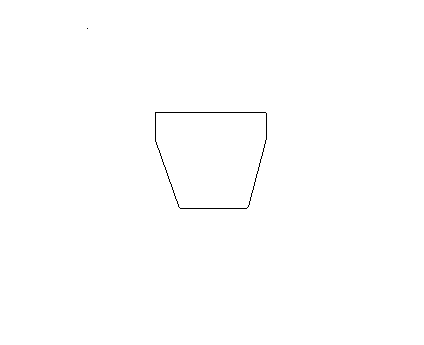
\includegraphics[scale=0.3]{borda.png}}
\subfigure[]{
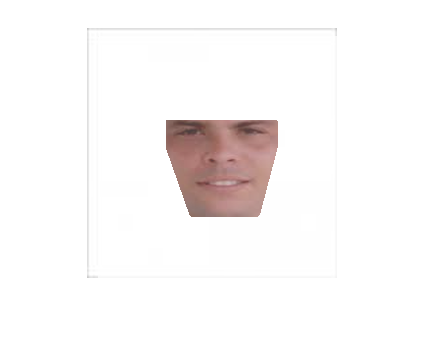
\includegraphics[scale=0.3]{covex_hull.png}}
\end{figure}

\end{frame}

%------------------------------------------------

\begin{frame}[fragile] % Need to use the fragile option when verbatim is used in the slide
\frametitle{Verbatim}
\begin{example}[Theorem Slide Code]
\begin{verbatim}
\begin{frame}
\frametitle{Theorem}
\begin{theorem}[Mass--energy equivalence]
$E = mc^2$
\end{theorem}
\end{frame}\end{verbatim}
\end{example}
\end{frame}

%------------------------------------------------

\begin{frame}
\frametitle{Figure}
Uncomment the code on this slide to include your own image from the same directory as the template .TeX file.
%\begin{figure}
%\includegraphics[width=0.8\linewidth]{test}
%\end{figure}
\end{frame}

%------------------------------------------------

\begin{frame}[fragile] % Need to use the fragile option when verbatim is used in the slide
\frametitle{Citation}
An example of the \verb|\cite| command to cite within the presentation:\\~

This statement requires citation \cite{p1}.
\end{frame}

%------------------------------------------------

\begin{frame}
\frametitle{References}
\footnotesize{
\begin{thebibliography}{99} % Beamer does not support BibTeX so references must be inserted manually as below
\bibitem[Smith, 2012]{p1} John Smith (2012)
\newblock Title of the publication
\newblock \emph{Journal Name} 12(3), 45 -- 678.
\end{thebibliography}
}
\end{frame}

%------------------------------------------------

\begin{frame}
\Huge{\centerline{The End}}
\end{frame}

%----------------------------------------------------------------------------------------

\end{document} 